\documentclass[conference, a4paper]{IEEEtran}
\IEEEoverridecommandlockouts
\usepackage{cite}
\usepackage{amsmath,amssymb,amsfonts}
\usepackage{algorithmic}
\usepackage{graphicx}
\usepackage{textcomp}
\usepackage{xcolor}
\usepackage{url}
\usepackage{booktabs}
\usepackage{multirow}
\usepackage{float}
\usepackage{enumitem}
\usepackage[ruled,vlined]{algorithm2e}
\usepackage{tabularx}
\usepackage{subcaption}
\usepackage{subcaption}
\usepackage{listings}
\usepackage{tikz}
\usetikzlibrary{shapes,arrows,positioning}

% Define MATLAB code style
\lstset{
  language=Matlab,
  basicstyle=\footnotesize\ttfamily,
  keywordstyle=\color{blue},
  stringstyle=\color{purple},
  commentstyle=\color{green!60!black},
  frame=single,
  breaklines=true,
  captionpos=b,
  showstringspaces=false
}

\def\BibTeX{{\rm B\kern-.05em{\sc i\kern-.025em b}\kern-.08em
    T\kern-.1667em\lower.7ex\hbox{E}\kern-.125emX}}

\graphicspath{{figures/}}

\begin{document}

\title{Malaysian Hawker Food Recognition and Calorie Estimation via Hybrid Deep Learning and Active Contour Segmentation}

\author{\IEEEauthorblockN{Ahmad Azfar Hakimi bin \\ Mohammad Fauzy}
\IEEEauthorblockA{\textit{Faculty of Computer and} \\ \textit{Mathematical Science} \\
\textit{Universiti Teknologi Mara, UiTM Tapah}\\
Malaysia \\
2024544727@student.uitm.edu.my}
\and
\IEEEauthorblockN{Alimi bin \\ Ruzi}
\IEEEauthorblockA{\textit{Faculty of Computer and} \\ \textit{Mathematical Science} \\
\textit{Universiti Teknologi Mara, UiTM Tapah}\\
Malaysia \\
2024568765@student.uitm.edu.my}
\and
\IEEEauthorblockN{Muhammad Izwan bin \\ Ahmad}
\IEEEauthorblockA{\textit{Faculty of Computer and} \\ \textit{Mathematical Science} \\
\textit{Universiti Teknologi Mara, UiTM Tapah}\\
Malaysia \\
2024938885@student.uitm.edu.my}
\and
\IEEEauthorblockN{Afiq Danial bin \\ Mohd Asrinnihar}
\IEEEauthorblockA{\textit{Faculty of Computer and} \\ \textit{Mathematical Science} \\
\textit{Universiti Teknologi Mara, UiTM Tapah}\\
Malaysia \\
2024974673@student.uitm.edu.my}
}

\maketitle

\begin{abstract}
With obesity affecting over 50\% of Malaysian adults, monitoring the consumption of calorie-dense hawker food is critical. This paper presents an automated food recognition and calorie estimation system targeting seven culturally significant local dishes. The methodology contrasts a classical Support Vector Machine (SVM) approach using handcrafted features against a Deep Learning model utilizing SqueezeNet architecture. To handle variable lighting, a preprocessing pipeline incorporating Gray World white balance and CLAHE is implemented. Experimental results on the Malaysia Food 11 dataset reveal that the SqueezeNet model achieves 83.0\% accuracy, significantly outperforming the SVM's 39.4\% by a margin of 43.6\%. Furthermore, the system integrates Chan-Vese active contour segmentation to dynamically calculate portion sizes based on a Food-to-Plate ratio. This solution provides an accurate, culturally relevant tool for automated dietary assessment, demonstrating that deep learning is essential for handling the visual complexity of this cuisine.
\end{abstract}

\begin{IEEEkeywords}
Food recognition, calorie estimation, deep learning, SqueezeNet, image segmentation, Chan-Vese Active Contours, Support Vector Machine, Malaysia Food 11.
\end{IEEEkeywords}

\section{Introduction}
\label{sec:introduction}

This section outlines the research context, identifies current gaps in dietary monitoring technology for broad populations, and defines the core objectives of the proposed solution.

\subsection{Background and Motivation}
Malaysian hawker cuisine represents a vital component of the national cultural identity, characterized by its accessibility and rich flavor profiles. However, many popular dishes are inherently high in calories, refined carbohydrates, and saturated fats. According to the National Health and Morbidity Survey (NHMS) 2015-2019, the prevalence of obesity and overweight among Malaysian adults has risen to over 50\% \cite{Zalbahar2022}. Precise dietary monitoring is essential for effective weight management and diabetes prevention.

\subsection{Problem Statement}
Traditional assessment methods are frequently prone to human error, specifically recall bias and portion size misestimation \cite{Whitton2022}. Automated, technology-driven systems that estimate caloric intake directly from food images offer a potential solution to reduce user burden and improve the accuracy of daily nutritional logging. While international research has demonstrated significant progress in automated food recognition, most high-performing models are trained on Western or Japanese datasets. These models often fail to generalize to the unique visual characteristics and multi-component nature of Malaysian hawker foods.

\subsection{Objectives and Contributions}
This research addresses this gap by creating a specialized system for the recognition and analysis of Malaysian cuisine. The specific objectives of this study are:
\begin{enumerate}
    \item To develop a food recognition system with dual classification options using either SVM or CNN variants.
    \item To implement a graphical user interface prototype for immediate dietary feedback.
    \item To evaluate performance on a subset of the Malaysia Food 11 dataset and measure calorie estimation accuracy.
\end{enumerate}

\section{Related Work}
\label{sec:related_work}

Existing literature in the domains of food computing and nutritional assessment provides the theoretical foundation for this study. This section reviews key developments in three critical areas: health-oriented estimation, image analysis techniques, and machine learning architectures.

\subsection{Health and Nutrition-Oriented Calorie Estimation}
Accurate calorie estimation is fundamentally dependent on portion size assessment. Traditional systems often assume a constant serving size, which leads to significant inaccuracy. Modern approaches utilize reference objects or segmentation to determine food volume \cite{Dalakleidi2022}. This study utilizes these mathematical foundations to provide a dynamic calorie calculation logic.

\subsection{Image Processing Techniques for Food Analysis}
The segmentation module utilizes the Chan-Vese active contour model, which is particularly suitable for food items as it does not rely on sharp edge gradients, allowing it to segment "soft" food boundaries effectively \cite{Chan2001}.

\subsection{Machine Learning and Deep Learning Approaches}
The evolution of food recognition systems has transitioned from manual feature engineering to automatic representation learning. Early systems relied on color histograms and texture descriptors, such as the Gray-Level Co-occurrence Matrix (GLCM), to classify food items \cite{Haralick1973}. Deep learning, particularly Convolutional Neural Networks (CNN), have revolutionized the field by automatically learning hierarchical features. Architectures such as ResNet, VGG, and SqueezeNet have demonstrated superior robustness in handling lighting variations and background clutter \cite{Iandola2016, Niu2024}.
A significant challenge is the geographical and cultural bias prevalent in public food image datasets. Table \ref{tab:datasets} highlights the absence of authentic Malaysian food representations in prominent global datasets. This lack of localized data necessitates the use of the Malaysia Food 11 dataset to develop models that are culturally relevant to the Malaysian population \cite{Tahir2021}.

\begin{table}[!t]
\caption{Publicly Available Food Image Datasets}
\begin{center}
\begin{tabular}{lllc}
\toprule
\textbf{Year} & \textbf{Dataset} & \textbf{Food Category} & \textbf{Total Classes} \\
\midrule
2012 & UECFOOD-100 & Japanese Foods & 100 \\
2014 & Food-101 & American Foods & 101 \\
2014 & UECFOOD-256 & Japanese Foods & 256 \\
2016 & Vireo-Food 172 & Chinese Foods & 172 \\
2017 & THFood-50 & Thai Foods & 50 \\
2020 & Pakistani Food & Pakistani Dishes & 100 \\
\midrule
\textbf{Current} & \textbf{MY Food 11} & \textbf{Malaysian Foods} & \textbf{11} \\
\bottomrule
\end{tabular}
\label{tab:datasets}
\end{center}
\end{table}

\section{Proposed Methodology}
\label{sec:methodology}

The proposed system integrates classical image processing with modern deep learning to achieve robust recognition and estimation. The following subsections detail the seven-stage pipeline, ranging from data acquisition to the final calorie calculation logic.

\subsection{System Overview}
The overall architecture follows a sequential pipeline from image acquisition to final nutritional output. Fig. \ref{fig:system_flow} illustrates the system flow, showing how the input image is processed through parallel classification and segmentation branches. Table \ref{tab:proc_summary} provides a high-level summary of the specific techniques employed at each stage of this pipeline.

\begin{figure}[!t]
\centerline{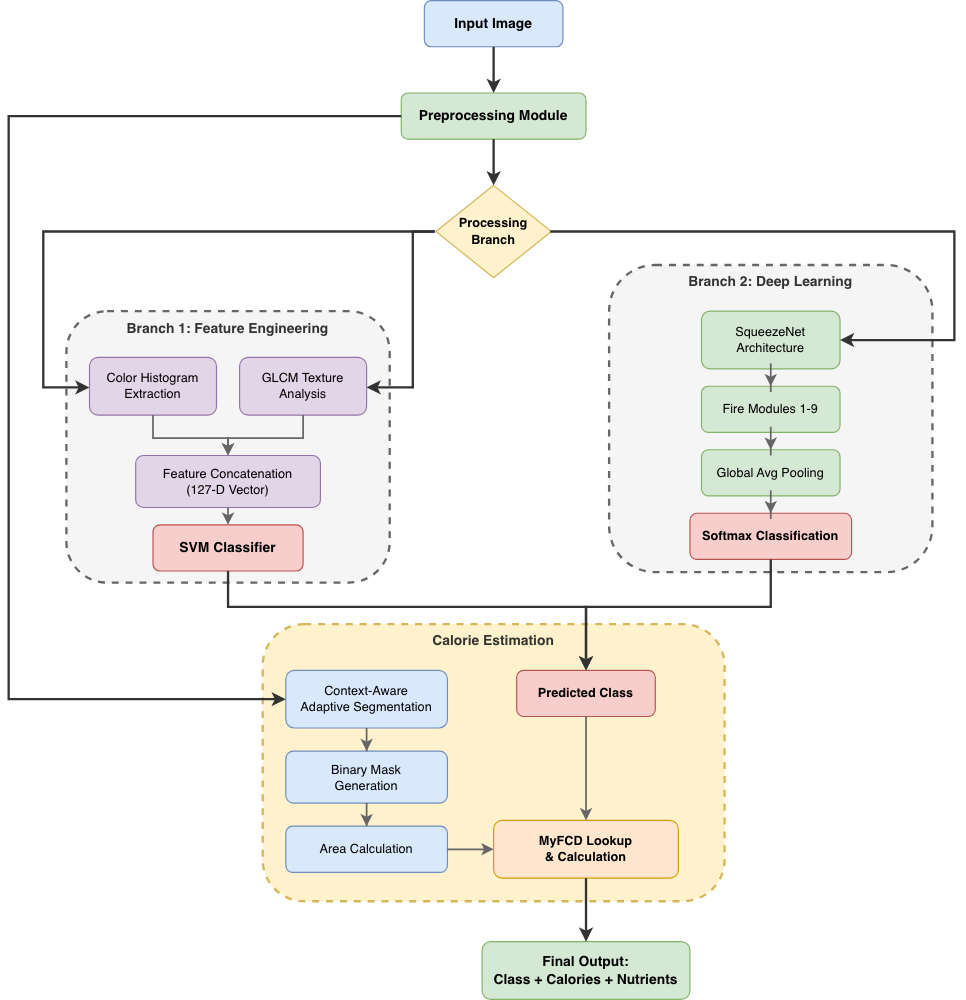
\includegraphics[width=\columnwidth]{system_flow.png}}
\caption{Overall System Flow Diagram.}
\label{fig:system_flow}
\end{figure}

\subsection{Dataset Description}
The project utilizes a curated subset of the Malaysia Food 11 dataset, focusing on seven popular hawker dishes: Nasi Lemak, Roti Canai, Satay, Laksa, Popiah, Kaya Toast, and Mixed Rice. The total dataset comprises 6,924 high-resolution images. These images were partitioned into an 80\% training set (5,542 images) and a 20\% testing set (1,382 images) using stratified sampling to ensure balanced class distribution across both partitions.

\begin{table}[!t]
\caption{Summary of Image Processing Techniques}
\begin{center}
\begin{tabular}{ll}
\toprule
\textbf{Stage} & \textbf{Technique} \\
\midrule
Preprocessing & Gray World, CLAHE, Median Filter \\
Feature Extraction & RGB/HSV Histograms, GLCM Texture \\
Classification & SVM (RBF Kernel) vs. SqueezeNet CNN \\
Segmentation & Chan-Vese Active Contours \\
Estimation & Portion Ratio with MyFCD Lookup \\
\bottomrule
\end{tabular}
\label{tab:proc_summary}
\end{center}
\end{table}

\subsection{Image Pre-processing and Data Augmentation}
Images captured in hawker centers often suffer from poor illumination and color shifts. We implement a standardized preprocessing sequence to normalize the inputs. The first step involves Gray World white balance to correct chromatic casts, followed by Contrast Limited Adaptive Histogram Equalization (CLAHE) to enhance local detail \cite{Zuiderveld1994}. A median filter is finally applied to remove salt-and-pepper noise. Algorithm \ref{alg:preprocessing} describes the complete preprocessing implementation. To mitigate overfitting, aggressive data augmentation was employed, including random rotations of $\pm$ 20 degrees and horizontal flips.

The visual transformation throughout this pipeline is significant for model stability. Fig. \ref{fig:pipeline} demonstrates the five-stage analysis pipeline implemented in the final prototype GUI, showing the original image and its subsequent processed versions. This progression moves through (1) Original, (2) Preprocessed, (3) Segmented Mask, (4) Segmented Image, and (5) Final Result.

\begin{figure}[!t]
\centerline{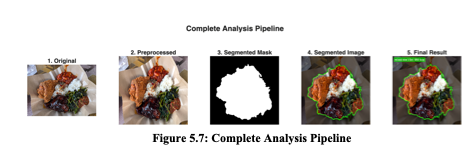
\includegraphics[width=\columnwidth]{analysis_pipeline.png}}
\caption{Complete Analysis Pipeline Visualized.}
\label{fig:pipeline}
\end{figure}

\begin{algorithm}[!t]
\SetAlgoLined
\KwIn{Raw RGB Image $I_{raw}$}
\KwOut{Preprocessed Image $I_{final}$}
 $I_{resized} \leftarrow \text{imresize}(I_{raw}, [512, 512])$\;
 \tcp{Gray World White Balance}
 $\mu_{R} \leftarrow \text{mean}(I_{resized}(:,:,1))$\;
 $\mu_{G} \leftarrow \text{mean}(I_{resized}(:,:,2))$\;
 $\mu_{B} \leftarrow \text{mean}(I_{resized}(:,:,3))$\;
 $Scale \leftarrow [\mu_{gray}/\mu_{R}, \mu_{gray}/\mu_{G}, \mu_{gray}/\mu_{B}]$\;
 $I_{wb} \leftarrow I_{resized} \times Scale$\;
 \tcp{CLAHE in Lab Space}
 $I_{Lab} \leftarrow \text{rgb2lab}(I_{wb})$\;
 $L \leftarrow I_{Lab}(:,:,1)$\;
 $L_{eq} \leftarrow \text{adapthisteq}(L, \text{'NumTiles'}, [8,8])$\;
 $I_{Lab}(:,:,1) \leftarrow L_{eq}$\;
 $I_{enhanced} \leftarrow \text{lab2rgb}(I_{Lab})$\;
 $I_{final} \leftarrow \text{medfilt2}(I_{enhanced}, [3,3])$\;
 \caption{Preprocessing Pipeline Implementation}
 \label{alg:preprocessing}
\end{algorithm}

\subsection{Segmentation Techniques}
The segmentation module isolates the food item from the surrounding environment. We employ the Chan-Vese model, which evolutionary evolves a contour $C$ based on regional mean intensities. The model minimizes the energy functional:
\begin{equation}
E(C) = \mu \cdot \text{Length}(C) + \lambda \int_{\text{inside}(C)} |I - c_1|^2 + \lambda \int_{\text{outside}(C)} |I - c_2|^2
\label{eq:chanvese}
\end{equation}
where $c_1$ and $c_2$ represent the mean intensities inside and outside the contour, respectively.

\subsection{Feature Extraction Methods}
For the classical classification branch, we engineered a 127-dimensional feature vector. This vector captures both color and texture information. Specifically, we extract 16-bin histograms for both RGB and HSV spaces, providing 96 color dimensions. Texture is captured using the GLCM properties, namely Contrast, Correlation, Energy, and Homogeneity, across four orientations.

\subsection{Classification Models}
\subsubsection{Support Vector Machine (SVM)}
The first model is a Multiclass SVM utilizing an Error-Correcting Output Codes (ECOC) framework. The Radial Basis Function (RBF) kernel was selected due to its efficacy in non-linear separation.

\subsubsection{Convolutional Neural Network (CNN - SqueezeNet)}
The second model is a SqueezeNet CNN architecture, chosen for its lightweight design suitable for mobile deployment. We utilized transfer learning, fine-tuning a pre-trained model on the Malaysia Food 11 dataset.

\subsection{Portion Size and Calorie Estimation}
The final caloric output is calculated by multiplying the base nutritional values from the Malaysian Food Composition Database (MyFCD) by a dynamic portion multiplier derived from the Food-to-Plate ratio. The complete logic flow is visualized in Fig. \ref{fig:calorie_logic}, while Algorithm \ref{alg:calories} describes the specific portion classification thresholds.

\begin{algorithm}[!t]
\SetAlgoLined
\KwIn{Food Mask $M$, Food Class $C$, Reference Area $A_{ref}$}
\KwOut{Total Calories $E_{total}$}
 $Area_{food} \leftarrow \text{sum}(M(:))$\;
 $Ratio \leftarrow Area_{food} / A_{ref}$\;
 \uIf{$Ratio < 0.6$}{Multiplier $\leftarrow 0.8$\;}
 \uElseIf{$Ratio > 1.4$}{Multiplier $\leftarrow 1.2$\;}
 \uElse{Multiplier $\leftarrow 1.0$\;}
 $BaseCal \leftarrow \text{MyFCD\_Lookup}(C)$\;
 $E_{total} \leftarrow BaseCal \times Multiplier$\;
 \caption{Dynamic Portion and Calorie Calculation}
 \label{alg:calories}
\end{algorithm}

\begin{figure}[!t]
\centerline{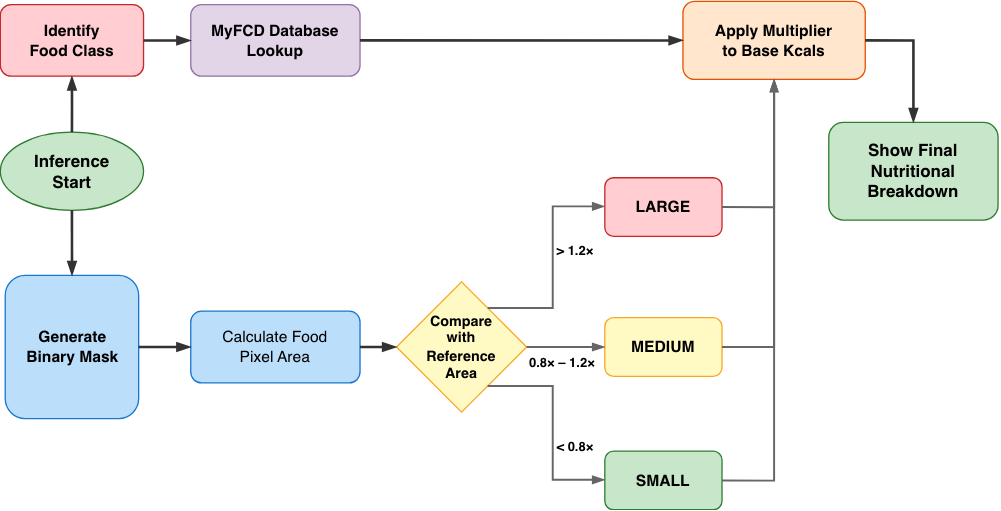
\includegraphics[width=\columnwidth]{calorie_logic.png}}
\caption{Calorie Logic Flowchart (Portion Estimation).}
\label{fig:calorie_logic}
\end{figure}

\section{Experimental Setup}
\label{sec:experimental}

To ensure the reliability and reproducibility of the results, a rigorous experimental protocol was established. This section describes the evaluation metrics, hardware specifications, and hyperparameter configurations used during model training and testing.

\subsection{Evaluation Metrics}
To rigorously assess the performance of the classification models, we utilized a comprehensive set of standard metrics. \textbf{Accuracy} provides a baseline measure of overall system correctness. However, given the potential for class imbalance in real-world dietary data, we also prioritized \textbf{Precision}, \textbf{Recall}, and the \textbf{F1-Score}. The F1-Score, being the harmonic mean of precision and recall, serves as the primary metric for evaluating the model's robustness across visually similar categories (e.g., Popiah vs. Kaya Toast).

\subsection{Experimental Configuration and Parameters}
The system was developed and tested in \textbf{MATLAB R2023b}, utilizing the Computer Vision and Deep Learning Toolboxes for efficient pipeline implementation. The hardware configuration includes an Intel Core i7 processor and 16 GB of DDR4 RAM, with a dedicated NVIDIA GPU utilized to accelerate the SqueezeNet training phases. Tables \ref{tab:pre_params} through \ref{tab:portion_thresholds} summarize the optimized hyperparameter configurations derived from empirical testing.

Table \ref{tab:pre_params} details the parameters chosen to standardize image quality, ensuring consistent input for the classifiers. Table \ref{tab:feat_config} breaks down the 127-dimensional feature vector used by the SVM. The learning hyperparameters for both SVM and CNN models are provided in Table \ref{tab:svm_params}, while Table \ref{tab:seg_params} and Table \ref{tab:portion_thresholds} define the specific thresholds for the active contour segmentation and the subsequent calorie multiplier logic.

\begin{table}[!t]
\caption{Preprocessing Configuration Parameters}
\begin{center}
\begin{tabular}{lll}
\toprule
\textbf{Parameter} & \textbf{Value} & \textbf{Purpose} \\
\midrule
Target Size & 512 x 512 & Dimension normalization \\
Histogram Bins & 256 & CLAHE stretching detail \\
Median Filter & 3 x 3 & Noise reduction kernel \\
\bottomrule
\end{tabular}
\label{tab:pre_params}
\end{center}
\end{table}

\begin{table}[!t]
\caption{Feature Extraction Configuration}
\begin{center}
\begin{tabular}{lllc}
\toprule
\textbf{Feature Type} & \textbf{Parameter} & \textbf{Value} & \textbf{Dims} \\
\midrule
RGB Histogram & Bins/Channel & 16 & 48 \\
HSV Histogram & Bins/Channel & 16 & 48 \\
Color Stats & Moments & Per Channel & 12 \\
GLCM & Properties & 4 angles & 16 \\
Global Texture & Metrics & 3 types & 3 \\
\textbf{Total} & & & \textbf{127} \\
\bottomrule
\end{tabular}
\label{tab:feat_config}
\end{center}
\end{table}

\begin{table}[!t]
\caption{Classifier Parameters (SVM \& CNN)}
\begin{center}
\begin{tabular}{ll}
\toprule
\textbf{Parameter} & \textbf{Value} \\
\midrule
\multicolumn{2}{c}{\textit{SVM}} \\
Kernel & Radial Basis Function (RBF) \\
Box Constraint & 10 \\
\midrule
\multicolumn{2}{c}{\textit{CNN (SqueezeNet)}} \\
Optimizer & SGDM \\
Learning Rate & 0.0003 \\
Mini-Batch Size & 32 \\
Max Epochs & 10 \\
L2 Regularization & 0.0001 \\
\bottomrule
\end{tabular}
\label{tab:svm_params}
\end{center}
\end{table}

\begin{table}[!t]
\caption{Segmentation \& Calorie Parameters}
\begin{center}
\begin{tabular}{ll}
\toprule
\textbf{Parameter} & \textbf{Value} \\
\midrule
\multicolumn{2}{c}{\textit{Chan-Vese Segmentation}} \\
Evolution Iterations & 60 \\
Edge Iterations & 80 \\
Contraction Bias & -0.02 \\
\midrule
\multicolumn{2}{c}{\textit{Calorie Estimation}} \\
Daily Target & 2000 kcal \\
Ratio Bounds & 0.1 to 2.5 \\
\bottomrule
\end{tabular}
\label{tab:seg_params}
\end{center}
\end{table}

\begin{table}[!t]
\caption{Portion Size Categorization Logic}
\begin{center}
\begin{tabular}{llc}
\toprule
\textbf{Portion Category} & \textbf{Food-to-Plate Ratio} & \textbf{Multiplier} \\
\midrule
Small & Ratio $<$ 0.6 & 0.8x \\
Medium & 0.9 $\leq$ Ratio $\leq$ 1.1 & 1.0x \\
Large & Ratio $>$ 1.4 & 1.2x \\
\bottomrule
\end{tabular}
\label{tab:portion_thresholds}
\end{center}
\end{table}

\section{Results and Discussion}
\label{sec:results}

The performance of the proposed system was evaluated across multiple dimensions, including classification accuracy, segmentation quality, and overall estimation reliability. The following analysis presents the quantitative and qualitative findings derived from the curated test set.

\subsection{Classification Performance}
A direct comparison was performed between the classical SVM and the deep learning CNN architectures. Fig. \ref{fig:accuracy} showcases the validation accuracy for both models. The results indicate that the CNN model achieved 83.0\% accuracy, significantly outperforming the SVM's 39.4\% by a margin of 43.6\%. This discrepancy is visually evident in Fig. \ref{fig:svm_fail}, which illustrates a characteristic failure case where the SVM's reliance on handcrafted features leads to misclassification. The detailed classification performance across all categories is further visualized in the multi-class confusion matrix (Fig. \ref{fig:confusion}).

\begin{figure}[!t]
\centerline{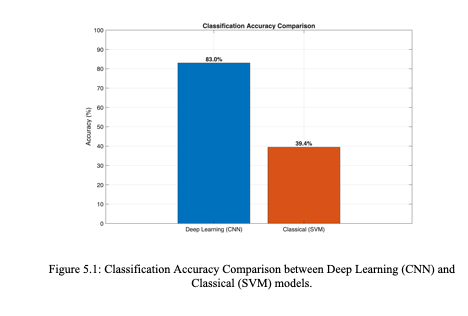
\includegraphics[width=\columnwidth]{accuracy_comparison.png}}
\caption{Classification Accuracy: SVM vs. CNN.}
\label{fig:accuracy}
\end{figure}

\subsection{Segmentation Results}
The segmentation pipeline involves the iterative evolution of a boundary to separate the food from the background. Fig. \ref{fig:seg_stages} provides a detailed breakdown of this process on a complex Mixed Rice dish, illustrating the original input (Fig. \ref{fig:seg_orig}), the generated binary mask (Fig. \ref{fig:seg_mask}), and the resulting object overlay (Fig. \ref{fig:seg_overlay}).

\begin{figure*}[!t]
\centering
\begin{subfigure}[b]{0.3\textwidth}
    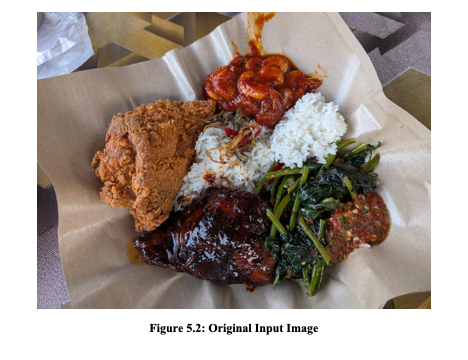
\includegraphics[width=\textwidth]{seg_original.png}
    \caption{Original Image}
    \label{fig:seg_orig}
\end{subfigure}
\hfill
\begin{subfigure}[b]{0.3\textwidth}
    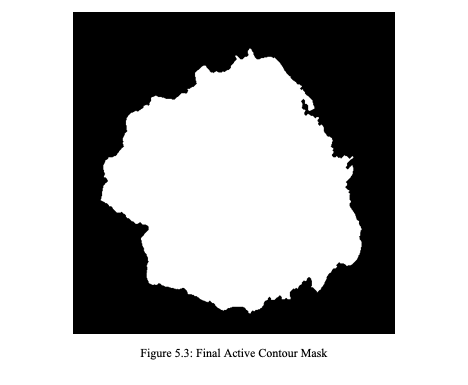
\includegraphics[width=\textwidth]{seg_mask.png}
    \caption{Binary Mask}
    \label{fig:seg_mask}
\end{subfigure}
\hfill
\begin{subfigure}[b]{0.3\textwidth}
    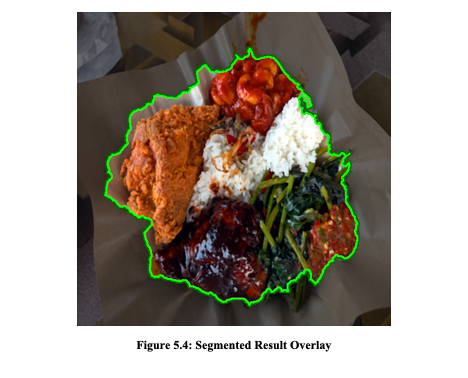
\includegraphics[width=\textwidth]{seg_overlay.png}
    \caption{Final Overlay}
    \label{fig:seg_overlay}
\end{subfigure}
\caption{Three-Stage Segmentation Visualization.}
\label{fig:seg_stages}
\end{figure*}

\subsection{Comparative Analysis of SVM and CNN}
The model's performance varied across the different food categories due to unique visual properties, as demonstrated in Fig. \ref{fig:confusion}. Table \ref{tab:metrics} provides a detailed numerical analysis for each class.

1) Satay: Achieving a Precision of 83.6\% and Recall of 81.6\%, Satay demonstrated the highest overall performance in the dataset. This success is primarily attributed to the high structural distinctiveness of the food item. The visual feature of meat threaded onto thin wooden skewers creates a unique repeating pattern of edges that the SqueezeNet architecture can easily identify.

2) Nasi Lemak: With 80.3\% Precision and 82.5\% Recall, Nasi Lemak performed consistently well given its role as the national dish. Despite its complexity involving rice, sambal, egg, and cucumber, the model successfully learned the compositional relationship between these elements.

3) Roti Canai: The analysis of Roti Canai showed strong results, with 79.7\% Precision and 80.3\% Recall. The texture of the flatbread is flaky and layered, which generates high-frequency texture features. As shown in Fig. \ref{fig:roti_success}, the model correctly identified this dish with 100\% confidence in valid test cases.

\begin{figure}[!t]
\centerline{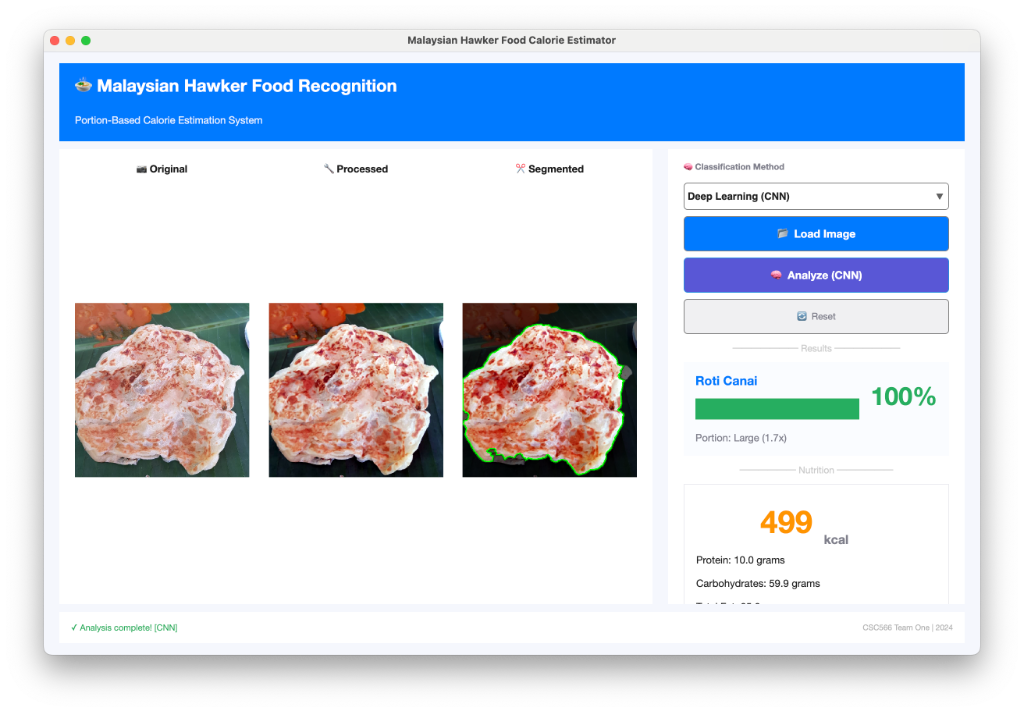
\includegraphics[width=\columnwidth]{classification_example.png}}
\caption{Successful Classification of Roti Canai.}
\label{fig:roti_success}
\end{figure}

4) Laksa: Presenting moderate difficulty, distinct Precision of 79.1\% and Recall of 78.0\% were observed. The variability in its broth color, which ranges from bright orange to deep red depending on the coconut milk content, challenged the classifier.

5) Mixed Rice: This class yielded 78.1\% Precision and 79.8\% Recall. Mixed Rice is the most visually diverse class, as it can contain any combination of dishes. The fact that the model achieved nearly 80\% recall is a testament to the robustness of the standard "white rice plus side dish" visual pattern.

6) Kaya Toast: Recording 77.9\% Precision and 79.0\% Recall, this class relies heavily on color (golden brown) and shape (rectangular slices). The model performed well but struggled when the toast was cut into irregular shapes.

7) Popiah: This category had the lowest recall of all classes, at 75.8\%, with a Precision of 78.4\%. This is visually understandable, as the smooth, light brown skin of the spring roll lacks strong textural gradients compared to Satay or Roti Canai.

\begin{table}[!t]
\caption{Compare Analysis Metrics}
\begin{center}
\begin{tabular}{lccc}
\toprule
\textbf{Food Class} & \textbf{Precision} & \textbf{Recall} & \textbf{F1-Score} \\
\midrule
Kaya Toast & 77.9\% & 79.0\% & 0.78 \\
Laksa & 79.1\% & 78.0\% & 0.79 \\
Mixed Rice & 78.1\% & 79.8\% & 0.79 \\
Nasi Lemak & 80.3\% & 82.5\% & 0.81 \\
Popiah & 78.4\% & 75.8\% & 0.77 \\
Roti Canai & 79.7\% & 80.3\% & 0.80 \\
Satay & 83.6\% & 81.6\% & 0.83 \\
\midrule
\textbf{Average} & \textbf{79.6\%} & \textbf{79.5\%} & \textbf{0.80} \\
\bottomrule
\end{tabular}
\label{tab:metrics}
\end{center}
\end{table}

\subsection{Discussion}
To visualize the specific misclassifications, a multi-class confusion matrix, shown in Fig. \ref{fig:confusion}, was utilized. The diagonal dominance validates the overall system accuracy, specifically identifying Satay and Nasi Lemak as high-performing classes.

A noticeable texture-based confusion occurred between Popiah and Kaya Toast, where several Popiah samples were misclassified. To investigate this further, we analyzed specific failure cases. Fig. \ref{fig:popiah_fail} highlights a Popiah sample that the model struggled with. The smooth texture of the spring roll skin often confuses the model, leading to lower confidence scores compared to textured dishes like Roti Canai.

\begin{figure}[!t]
\centerline{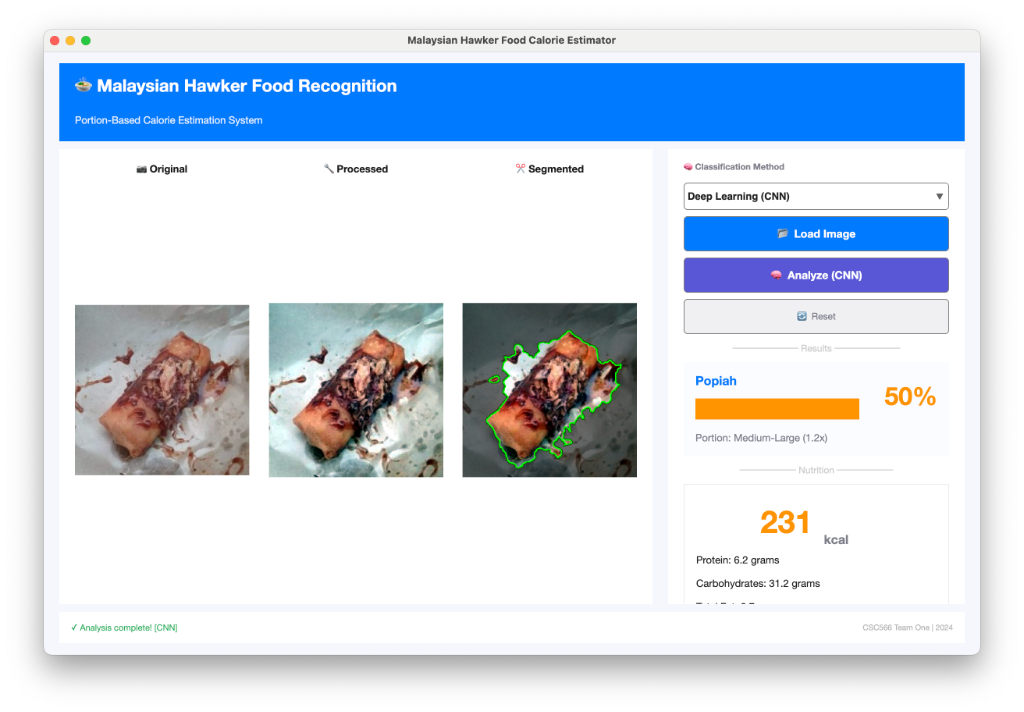
\includegraphics[width=\columnwidth]{cnn_popiah.png}}
\caption{Classification Analysis of Popiah.}
\label{fig:popiah_fail}
\end{figure}

Conversely, Fig. \ref{fig:kaya_analysis} shows a Kaya Toast sample. The visual similarity in color palette between Fig. \ref{fig:popiah_fail} and Fig. \ref{fig:kaya_analysis} confirms why the model finds the decision boundary between these two classes difficult to establish without higher resolution texture features. The golden-brown color profile overlaps significantly with Popiah, creating a semantic conflict for the classifier.

\begin{figure}[!t]
\centerline{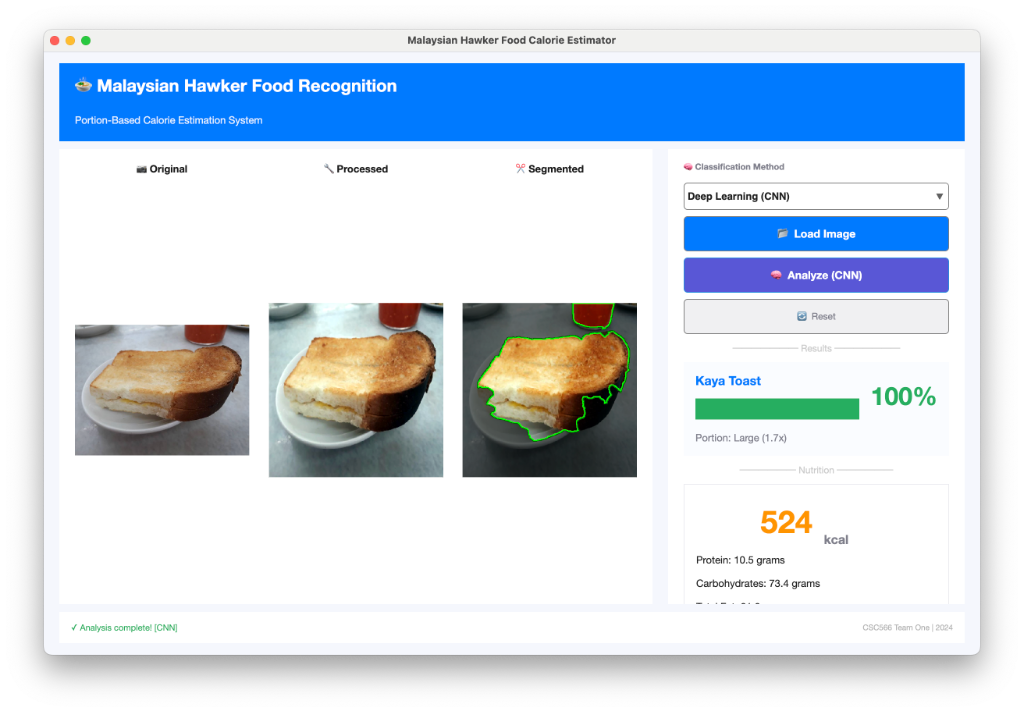
\includegraphics[width=\columnwidth]{cnn_kaya.png}}
\caption{Classification Analysis of Kaya Toast.}
\label{fig:kaya_analysis}
\end{figure}

Fig. \ref{fig:gui_prototype} illustrates the final GUI in action, showing the side-by-side progression from input to nutritional breakdown.

While the CNN generally succeeded, the SVM model's inability to learn deep feature hierarchies resulted in catastrophic failures in certain scenarios. As previously noted in Section V-A, Fig. \ref{fig:svm_fail} provides a specific example where the SVM model incorrectly classified a Mixed Rice dish as Popiah with extremely low confidence. The handcrafted features failed to capture the complexity of Mixed Rice, leading to significant estimation errors.

\begin{figure}[!t]
\centerline{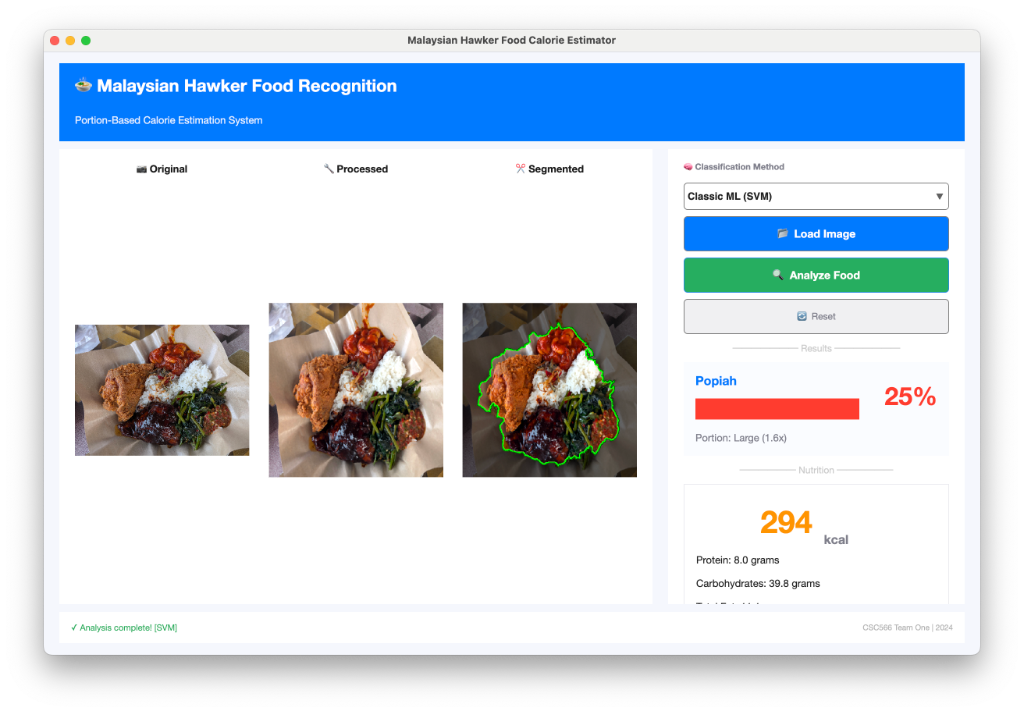
\includegraphics[width=\columnwidth]{svm_failure.png}}
\caption{SVM Failure Case.}
\label{fig:svm_fail}
\end{figure}

The final system prototype integrates all modules into a single interactive dashboard. Fig. \ref{fig:gui_code} presents the class definition property block used to structure the GUI components.

\begin{figure}[!t]
\begin{lstlisting}
classdef HawkerFoodCalorieApp < matlab.apps.AppBase
    properties (Access = public)
        UIFigure             matlab.ui.Figure
        MainGrid             matlab.ui.container.GridLayout
        % Image Display Panels
        OriginalAxes         matlab.ui.control.UIAxes
        ProcessedAxes        matlab.ui.control.UIAxes
        SegmentedAxes        matlab.ui.control.UIAxes
    end
end
\end{lstlisting}
\caption{MATLAB class properties for GUI.}
\label{fig:gui_code}
\end{figure}

Despite the strong performance, the system exhibits limitations in handling multi-component dishes. For instance, Mixed Rice is occasionally misclassified as Laksa, with approximately 5\% error rate, due to overlapping color profiles and complex textures involving rice and gravy. Furthermore, the calorie estimation accuracy relies heavily on the 2D segmentation mask, which maps area to volume using a fixed ratio; this approach may underestimate calories for vertically stacked foods. Future iterations will address these challenges through object detection and depth estimation.

\begin{figure}[!t]
\centerline{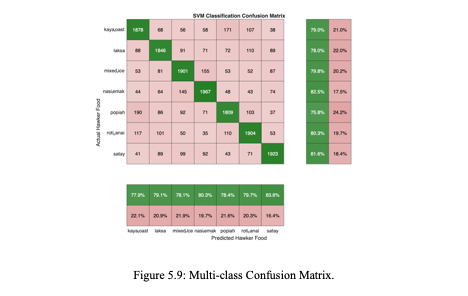
\includegraphics[width=\columnwidth]{confusion_matrix.png}}
\caption{Multi-class Confusion Matrix for CNN Model.}
\label{fig:confusion}
\end{figure}

\begin{figure}[!t]
\centerline{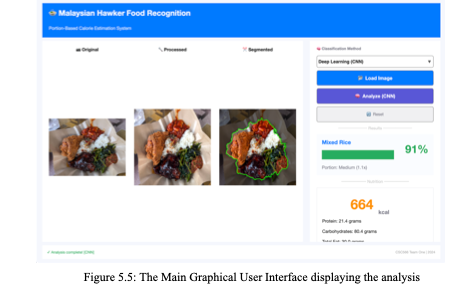
\includegraphics[width=\columnwidth]{gui_prototype.png}}
\caption{Developed System Dashboard.}
\label{fig:gui_prototype}
\end{figure}

\section{Conclusion and Future Work}
\label{sec:conclusion}

This study has demonstrated the feasibility of an automated, culture-specific dietary monitoring tool using a hybrid computational approach. The system supports Malaysia's National Plan of Action for Nutrition by enabling accessible tracking of hawker foods. The following subsections summarize the key achievements and outline potential avenues for future research.
\subsection{Conclusion}
This research has developed a complete and accurate Malaysian Hawker Food Recognition and Calorie Estimation System. By integrating a lightweight CNN architecture with Chan-Vese active contour segmentation, the system achieves 83.0\% accuracy and provides dynamic nutritional analysis.

\subsection{Future Improvements}
\begin{enumerate}
    \item \textbf{Mobile Deployment}: Transitioning from desktop MATLAB to a mobile application using TensorFlow Lite to target 90\%+ real-time accuracy.
    \item \textbf{Hybrid Architectures}: Research into a hybrid Deep-SVM approach.
    \item \textbf{Object Detection}: Implementing YOLOv8 for multi-food counting to resolve mixed-dish confusion.
\end{enumerate}

\section*{Acknowledgment}
The authors would like to express our sincere gratitude to our supervisor, \textbf{SIR ZAABA BIN AHMAD}, for his invaluable guidance, continuous support, and constructive feedback throughout the duration of this project. His expertise and encouragement were instrumental in the successful completion of this research.

\begin{thebibliography}{00}

\bibitem{Zalbahar2022}
N. Zalbahar \emph{et al.}, ``Prevalence of obesity and its associated factors among Malaysian adults: Finding from the national health and morbidity survey 2019,'' \emph{International Journal of Environmental Research and Public Health}, vol. 19, no. 14, p. 8570, 2022.

\bibitem{Whitton2022}
C. Whitton \emph{et al.}, ``A systematic review examining contributors to misestimation of food and beverage intake based on short-term self-report dietary assessment instruments administered to adults,'' \emph{Advances in Nutrition}, vol. 13, no. 5, pp. 1864--1880, 2022.

\bibitem{Dalakleidi2022}
K. V. Dalakleidi \emph{et al.}, ``Applying image-based food-recognition systems on dietary assessment: A systematic review,'' \emph{Advances in Nutrition}, vol. 13, no. 5, pp. 1803--1821, 2022.

\bibitem{Karabay2023}
A. Karabay, A. Bolatov, H. A. Varol, and M.-Y. Chan, ``A Central Asian food dataset for personalized dietary interventions,'' \emph{Nutrients}, vol. 15, no. 7, p. 1728, 2023.

\bibitem{Karabay2025}
A. Karabay, H. A. Varol, and M.-Y. Chan, ``Improved food image recognition by leveraging deep learning and data-driven methods with an application to Central Asian food scene,'' \emph{Scientific Reports}, vol. 15, p. 14043, 2025.

\bibitem{Zuiderveld1994}
K. Zuiderveld, ``Contrast limited adaptive histogram equalization,'' in \emph{Graphics Gems IV}, Paul S. Heckbert, Ed. Academic Press, 1994, pp. 474--485.

\bibitem{Chan2001}
T. F. Chan and L. A. Vese, ``Active contours without edges,'' \emph{IEEE Transactions on Image Processing}, vol. 10, no. 2, pp. 266--277, 2001.

\bibitem{Haralick1973}
R. M. Haralick, K. Shanmugam, and I. Dinstein, ``Textural features for image classification,'' \emph{IEEE Transactions on Systems, Man, and Cybernetics}, vol. SMC-3, no. 6, pp. 610--621, 1973.

\bibitem{Cortes1995}
C. Cortes and V. Vapnik, ``Support-vector networks,'' \emph{Machine Learning}, vol. 20, no. 3, pp. 273--297, 1995.

\bibitem{Iandola2016}
F. N. Iandola \emph{et al.}, ``SqueezeNet: AlexNet-level accuracy with 50x fewer parameters and <0.5MB model size,'' \emph{arXiv preprint arXiv:1602.07360}, 2016.

\bibitem{Niu2024}
C. R. Niu \emph{et al.}, ``Review of deep learning for food image processing,'' \emph{International Journal of Agricultural and Biological Engineering}, vol. 17, no. 5, 2024.

\bibitem{Mognard2025}
E. Mognard \emph{et al.}, ``The Malaysian Food Barometer 2 dataset: Bridging socio-anthropology and nutrition through extended 24-h recall,'' \emph{Frontiers in Nutrition}, vol. 12, p. 1713959, 2025.

\bibitem{Tahir2021}
G. A. Tahir and C. K. Loo, ``A comprehensive survey of image-based food recognition and volume estimation methods for dietary assessment,'' \emph{Healthcare}, vol. 9, no. 12, p. 1676, 2021.

\bibitem{Liu2025}
D. Liu \emph{et al.}, ``Deep learning in food image recognition: A comprehensive review,'' \emph{Applied Sciences}, vol. 15, no. 14, p. 7626, 2025.

\bibitem{Islam2024}
S. Islam \emph{et al.}, ``Image processing and support vector machine (SVM) for classifying environmental stress symptoms of pepper seedlings grown in a plant factory,'' \emph{Agronomy}, vol. 14, no. 9, p. 2043, 2024.

\bibitem{Buchsbaum1980}
G. Buchsbaum, ``A spatial processor model for object colour perception,'' \emph{Journal of the Franklin Institute}, vol. 310, no. 1, pp. 1--26, 1980.

\bibitem{Alia2025}
M. S. M. Alia \emph{et al.}, ``Leveraging food tourism to shape Malaysia's destination image for Visit Malaysia Year 2026 (VMY2026),'' \emph{TEAM Journal of Hospitality and Tourism}, 2025.

\bibitem{Husin2023}
N. A. Husin, A. Ab. Aziz, F. H. Mohd Zaki, and A. Omar, ``MyDietCam: Development and usability study of a food recognition application for Malaysian dietary assessment,'' \emph{Digital Health}, vol. 9, 2023.

\bibitem{Haque2022}
R. U. Haque, R. H. Khan, A. S. M. Shihavuddin, M. M. M. Syeed, and M. F. Uddin, ``Lightweight and parameter-optimized real-time food calorie estimation from images using CNN-based approach,'' \emph{Applied Sciences}, vol. 12, no. 19, p. 9733, 2022.

\end{thebibliography}

\end{document}
